\documentclass[11pt]{article}
\usepackage[margin=1.15in]{geometry}
\usepackage{amsmath,amssymb,amsthm}
\usepackage{enumitem}
\usepackage{graphicx}
\usepackage{tikz}
\usetikzlibrary{positioning,fit,arrows,calc}
\usepackage[hidelinks]{hyperref}
\setlength{\parindent}{1.5em}
\setlength{\parskip}{0.3em}
\linespread{1.08}

\newtheorem{proposition}{Proposition}
\theoremstyle{definition}
\newtheorem{definition}{Definition}
\newtheorem{principle}{Principle}

\title{Issuance Against Improvement:\\A Monetary Theory of Certified Built Capacity}
\author{Flyxion\\\small Independent Researcher}
\date{October 2026}

\begin{document}
\maketitle

\begin{abstract}
\noindent This essay develops a monetary and credit architecture in which financial claims originate from certified, location-indexed physical improvements to the built environment and not from the market price of real estate. A first formulation takes the form of a currency, the Built Capacity Unit, issued against certified quantities of lawful built capacity. The essay formalizes that formulation, separates it into three ideas (an issuance rule, a code-based verification ontology, and a spatial topology), and follows each through the objections that formalization raises. The analysis moves through four stages: property-backed money, capacity-backed money, transformation-backed credit, and an attestation-based collateral architecture. The first stage is the familiar mortgage-backed regime. The second fails for want of a numeraire, because it cannot say who bears the destruction of backing, and because it lets legislative zoning act as a source of issuance. The third replaces the stock of capacity by the attested transformation as the primitive object, and issues amortizing credit against replacement-cost increments. The fourth observes that what survives is better described as underwriting information than as monetary backing, and that it can be built with no new currency at all. The resulting design is distinguished from blockchain systems by the problem it addresses, warrant for records and not agreement about records. Location, on this account, belongs in the provenance of a financial claim and not in the denomination of money, and building codes can determine whether a transformation is admissible collateral without determining how much money an economy should possess. The essay also argues that rule-based issuance is not discretion-free issuance, since discretion migrates upstream into the definition, measurement, and certification of eligible transformations, and it sets out a nested hierarchy of institutional systems of which only the weakest need be established for the core idea to hold.
\end{abstract}

\section{The Idea and Its Three Components}

The idea developed here begins from the observation that a building joins three things which monetary theory ordinarily treats separately: a location, a durable physical capital good, and a bundle of legally defined obligations that determine what the capital good is permitted to be. From this a first formulation develops a currency unit, provisionally the Built Capacity Unit, issued against standardized quantities of certified lawful built capacity. A parcel has a legally permitted state space, fixed by zoning, setbacks, servicing requirements, fire and structural rules, accessibility provisions, and occupancy classifications. The regulations that ordinarily appear as restrictions on use are reinterpreted as the definition of an economically measurable resource. The certified capacity at a location $x$ is written
\begin{equation}
C(x) \;=\; A(x)\,Q(x)\,L(x),
\label{eq:capacity}
\end{equation}
where $A$ is permitted usable floor area, $Q$ is a code-compliance or infrastructure factor, and $L$ is a location coefficient intended to be built from physical quantities (access to roads, utilities, transit, emergency services, employment catchments, water and sewer capacity, climate risk, replacement cost) instead of from speculative land prices. The monetary base is then related to certified capacity by
\begin{equation}
M \;=\; \alpha \sum_{x} C(x), \qquad 0<\alpha<1,
\label{eq:base}
\end{equation}
so that only a fraction of certified capacity supports circulating claims.

Three distinct ideas are bundled in this construction, and the case for or against each is easier to assess once they are separated. The first is an \emph{issuance rule}: new money may be created when capacity is created, and not when the exchange price of existing capacity rises. The second is a \emph{verification ontology}: the objects against which issuance occurs are defined by a public code, and the attestation that they exist is a narrow factual claim about a transformation, not a valuation. The third is a \emph{topology}: claims are not spaceless entries in a ledger but propagate through a graph $G=(V,E)$ whose vertices are parcels, blocks, municipalities, or servicing zones and whose edges are roads, utilities, commuting relations, watersheds, or jurisdictions. Each of the three can be adopted without the others, and each has different strengths.

The argument that follows has a definite direction, and it is worth stating at the outset so that the intermediate difficulties can be read as stages of a single movement. The first formulation is a theory of money as a function of things: how much money a building, or a quantity of certified capacity, should contain. The analysis finds that this question is badly posed. The numeraire is missing, the stock of capacity decays and is destroyed, and the legal definition of capacity is itself a legislative variable. What replaces it is a theory of credit as a function of verified changes to things. The question that organizes the reformulation is the following.

\begin{quote}
The central design problem is not how much money a building should contain, but what monetary claims a verified transformation of the built environment should be permitted to originate.
\end{quote}

\noindent Sections 2 through 8 examine the first formulation, and Section 6 separates the design from blockchain systems, which it resembles architecturally and differs from in the verification problem it addresses, and Section 9 states the reformulation that results. Sections 10 and 11 treat the institutional questions the reformulation makes unavoidable: who holds the discretion that the rule conceals, and how the design nests within a spectrum of weaker and stronger institutional commitments. Section 12 reports four dimensionless illustrative simulations of the feedback, destruction, cost, and clearing mechanisms discussed along the way.

\section{What the Capacity Formulation Gets Right}

The strongest feature of the capacity formulation is its treatment of the feedback loop in conventional property finance. In the ordinary arrangement, a rise in the price of land permits larger loans against that land, larger loans increase the purchasing power available to buyers, and increased purchasing power supports further rises in price. Household balance-sheet evidence from the United States is consistent with the first link of this chain, since borrowing against rising home equity expanded household leverage \cite{mian2011}. This is the collateral channel familiar from the credit-cycle literature, in which asset prices and borrowing capacity amplify one another \cite{kiyotaki1997, bernanke1989}, and the long historical record of mortgage lending suggests that the channel has become quantitatively central to modern financial systems \cite{jorda2016, knoll2017, schularick2012}. The formulation cuts the loop at a specific point. If monetary capacity is created only against an increase in certified physical capacity, then a neighbourhood that becomes fashionable and sees land prices double has not thereby created any new capacity, and no new money issues. A foundation replaced, an apartment added, a sewer line extended, or twenty compliant houses constructed all raise certified capacity, and each is a physical and administratively verified event. The aphorism that nothing physically changed, therefore nothing monetary changed, is a clean statement of a design principle, and it is not trivially satisfied by existing systems.

The second strength is the narrowness of the attestation. An inspector in this scheme is not asked what a property is worth, which would reintroduce the appraisal and with it the same reflexive dependence on current bids. The inspector is asked whether a specified transformation occurred and whether the resulting structure satisfies publicly stated conditions. Propositions of this form are checkable by a third party in a way that valuations are not. Two houses of nearly identical structural capacity, one priced at a multiple of the other because of where it stands, are physically near-equivalent, and a system that tracks improvement does not treat the scarcity premium on the second as a physical fact about it. It would be a mistake to conclude from this that the two houses must generate identical issuance. Capacity equivalence and issuance equivalence are different relations, and the second depends on the reproduction cost of the transformation, which can differ between places for reasons that have nothing to do with scarcity rent. That distinction is developed in Section 9; for the moment it suffices to note that the attraction of the design is the exclusion of scarcity rent from issuance, not the equalization of issuance across all physically similar buildings.

The third strength is philosophical but has operational content. A ledger in which each entry must trace to a located, inspected, permitted physical event is a ledger that cannot float indefinitely free of the territory it claims to describe. The chain
\begin{equation}
\text{parcel} \to \text{permit} \to \text{materials and work} \to \text{inspection} \to \text{occupancy} \to \text{capacity credit}
\label{eq:chain}
\end{equation}
is a provenance structure of the kind that makes forgery costly and audit possible \cite{buneman2001}. It replaces the scarcity-by-expenditure of proof-of-work, and the scarcity-by-ownership of proof-of-stake, with a scarcity-by-admissible-transformation that is anchored in institutions already present in most jurisdictions. The comparison with cryptographic ledgers is, however, less apt than the comparison with the cadastre. Land registries and cadastral surveys have long been the means by which states make parcels legible and attach rights and obligations to them \cite{scott1998}, and the registration of those rights has been argued to determine whether physical assets can serve as collateral at all \cite{desoto2000}. The structure in~\eqref{eq:chain} is best understood as a cadastral register augmented with append-only records of permitted and inspected transformations. The innovation is therefore not the existence of records tied to parcels. It is the coupling of a cadastre, a code-indexed attestation of transformations, a replacement-cost valuation, and a rule for credit creation. These features justify taking the idea seriously. They do not yet establish that it constitutes a monetary system, and the next sections examine where it is underdetermined.

\section{The Missing Numeraire}

Equation~\eqref{eq:base} equates a quantity of money with a fraction of a sum of capacities, but $C(x)$ as defined in~\eqref{eq:capacity} has no stated unit that can be converted into currency. Floor area multiplied by two dimensionless factors is an area, perhaps weighted. To write $M=\alpha\sum_x C(x)$ one must supply a conversion constant with dimensions of currency per unit weighted area, and that constant is exactly the object the system needs to explain. If it is set by administrative decree, the unit is a fiat unit with a collateral rule attached. If it is set by reference to market prices of floor space, the appraisal channel has been reintroduced through the back door. If it is set by replacement cost, the unit is anchored to the current cost of reproducing the capacity, which is a more defensible choice and is developed in Section~\ref{sec:repair}. The first formulation defers the central question of what determines the price level, and this deferral is not innocuous.

A related difficulty is that equation~\eqref{eq:base} makes the money supply a function of the supply side of the capacity economy alone. In ordinary monetary theory the quantity of money that an economy requires depends on the volume and velocity of transactions it must settle, and a currency whose supply is rigidly tied to a slow-moving physical stock will be badly matched to a demand for transactions balances that moves quickly. The historical analogue is instructive. John Law's early eighteenth-century proposal for land-backed paper money \cite{law1705} reasoned that money issued against land would be secure because land is durable, and the later fate of schemes of this kind turned on exactly this mismatch between a fixed-seeming collateral base and a variable need for circulating medium. The doctrine that money should be issued against real productive assets so that its supply tracks real activity has a long lineage under the label of the real bills doctrine \cite{mints1945}, and its standard difficulty is that the quantity of eligible assets is not independent of the price level that the money itself helps determine \cite{sargent1982}. A built-capacity currency avoids part of this circularity, because physical capacity is less sensitive to current bids than commercial paper is, but it does not escape the requirement that some mechanism connect the money supply to the demand for money. Without that mechanism the system will tend toward either chronic scarcity of medium, if capacity grows slowly, or toward an inflation concentrated in whichever regions happen to be building.

\section{Site and Improvement Are Not Cleanly Separable}

The most attractive formal move in the first formulation is the decomposition of each parcel into a pair
\begin{equation}
P(x) \;=\; (S_x, I_x),
\label{eq:pair}
\end{equation}
in which $S_x$ is scarce spatial privilege and $I_x$ is certified improvement, with issuance permitted against increments of $I_x$ and prohibited or limited against increments of $S_x$. This is a monetary application of the distinction that Henry George placed at the centre of his political economy \cite{george1879}, and it inherits both the force of that distinction and its characteristic difficulty. The difficulty is that the value of an improvement is not independent of the site on which it stands, and the value of a site is not independent of the improvements and public works that surround it. A sewer line extended to a parcel raises the certified improvement on that parcel, and it also changes the set of uses the site can support, which is a change in what the formulation calls spatial privilege. An upgraded transit connection is a public improvement that raises the location coefficient $L$ of every parcel it serves, and the formulation's own construction of $L$ from access to transit, utilities, and emergency services makes the location coefficient a function of precisely the public investments whose effect the decomposition was meant to exclude from monetary creation.

The non-separability can be stated precisely. Let the exchange value of a parcel be $V(x)$ and suppose it is written
\begin{equation}
V(x) \;=\; S_x + I_x + J_x,
\label{eq:interaction}
\end{equation}
where $J_x$ is an interaction term capturing the extent to which the value of the improvement depends on the site and conversely. If $J_x\equiv 0$ the decomposition is exact and the issuance rule is well defined. In general $J_x\neq 0$, and an increment $\Delta I_x$ in certified improvement will be accompanied by an increment $\Delta J_x$ whose attribution to improvement or to site is a matter of convention. The practical consequence is that the issuance rule requires an explicit convention for attributing interaction value, and different conventions will produce different monetary expansions from the same physical event. A Georgist convention would assign interaction value to the site and issue only against the reproduction cost of the structure itself. A development-oriented convention would assign it to the improvement and issue more freely. Neither is natural, and the choice between them is a policy decision about who captures the gains from complementarity, not a measurement.

There is a useful result in the public-finance literature that bears on this point. Under idealized conditions, aggregate land rent in a city of optimal size is just sufficient to finance the public goods that make the land valuable \cite{arnott1979}. The implication is that the site-value component $S_x$ is in significant part a capitalization of public investment, and that a monetary system which refuses to issue against $S_x$ is in effect refusing to issue against the capitalized value of infrastructure that the community has already paid for. This is a coherent policy position, and it is arguably the Georgist position, but it should be stated as a position and not presented as an incidental consequence of the measurement scheme. The empirical record on taxing land more heavily than structures is limited, though one frequently cited study of a United States city found increased building activity after a shift toward land taxation \cite{oates1997}. The repair is to define issuance against the \emph{replacement cost} of the certified improvement, a quantity that can be estimated from construction cost indices and that does not move with the bids of purchasers, and to treat interaction value as unissued. This sacrifices some of the elegance of~\eqref{eq:capacity} and gains a measurable, auditable base.

\section{Codes as Ontology and as Target}

The observation that building codes contain a primitive ontology of real economic things is correct and underappreciated. Codes distinguish habitable rooms from non-habitable ones, specify egress, load paths, fire separations, ventilation rates, and electrical service capacity, and they do so in terms that are operational enough to be checked. These are harder to inflate rhetorically than a generic appraisal. The very property that makes codes useful for verification also makes them unstable as a monetary foundation, and three difficulties follow.

First, certified capacity is a function of the code edition in force, so the same structure can have different certified capacity under different editions. Write the certified capacity of structure $s$ under code edition $\kappa$ as $C_\kappa(s)$. A tightening of the code from $\kappa$ to $\kappa'$ may reduce $C_{\kappa'}(s)$ for existing structures that were compliant under $\kappa$, and a loosening may increase it. Because code editions are produced by legislative and administrative processes, the monetary system would inherit, as a source of discretionary shocks, every amendment cycle of every jurisdiction in which it operates. Grandfathering provisions can blunt this effect for individual structures, but a grandfathered structure has certified capacity that is a historical artifact, and the ledger must then record not only the physical state but the edition against which it was certified.

\begin{definition}[Indexed attestation]
An attestation is a tuple $(x, \tau, \kappa, \sigma, t)$ consisting of a location $x$, a transformation $\tau$ applied to that location, a code edition $\kappa$, a signed inspection record $\sigma$, and a time $t$. The certified capacity of a location at time $t$ is a function of the sequence of attestations at that location indexed by edition, and is defined only relative to a stated edition.
\end{definition}

Second, zoning and permitted floor area are themselves instruments of public policy, and an upzoning that increases $A(x)$ by legislative act raises certified capacity without any physical transformation. The governing principle is that issuance should follow physical change and not price change, but a zoning amendment is neither. It is a change in the legally permitted state space, and the first formulation would treat it as creating monetary capacity. This is the most serious internal contradiction in the first formulation, because the political incentives it creates are obvious: a jurisdiction that wishes to expand its money supply may do so by relaxing the permitted state space, and the owners of affected parcels acquire a claim on newly issued currency by lobbying. Municipalities could in effect print backing by redrawing zoning maps. Land-use regulation is, moreover, a significant determinant of local housing costs and of how responsive housing supply is to demand \cite{glaeser2003, gyourko2008}, so permitted capacity is not a neutral bookkeeping variable. The repair distinguishes \emph{permitted} capacity from \emph{realized} capacity and issues only against the latter, so that a zoning change creates an option but no issuance event. Capacity that is permitted and unbuilt is an entitlement; capacity that is built and certified is the base for credit. This is stated formally in Section~\ref{sec:repair} as the second of the proposition-level results, and it is the exact sense in which legislative expansion of the state space cannot by itself produce issuance.

Third, any measure that becomes the object of reward is subject to the familiar pattern in which the measure ceases to track the property it was chosen to represent, usually stated in the form attributed to Goodhart \cite{goodhart1975} and elaborated by Campbell \cite{campbell1979} and Strathern \cite{strathern1997}, with a book-length treatment of the costs of metric fixation in \cite{muller2018}. The general statement is less useful than a worked case, and the case can be given in the present setting. Suppose issuance rewards certified habitable floor area, and verification samples insulation, fire separation, and egress. A developer now faces the problem of maximizing credit eligibility, not social or service value. Writing $\Delta M(\tau)$ for the credit a transformation $\tau$ qualifies for and $U(\tau)$ for the actual value of the improvement to its occupants and to the surrounding community, the developer solves
\begin{equation}
\max_{\tau}\ \Delta M(\tau) \qquad\text{rather than}\qquad \max_{\tau}\ U(\tau),
\label{eq:goodhart}
\end{equation}
and the divergence between the two objectives is the concrete form of the problem. Cheap qualifying floor area is maximized; costly characteristics that are weakly represented in the certification function, such as the durability of concealed structural members or the quality of work that is expensive to reach, are minimized; and compliance effort is concentrated on components that the sampling procedure is likely to inspect. The monetary system pays for the optimization. This is not an argument against codes as a basis for verification, which are no worse in this respect than any other measurable standard, but it is an argument for treating the inspection regime as an adversarial institution. The inspector is an oracle in the technical sense: the ledger trusts an off-ledger observation, and the integrity of the credit it supports is bounded above by the integrity of that observation. The design must therefore include rotation, sampling audits whose sampling is not predictable by the builder, liability for false attestation, and the possibility of post hoc challenge, with the credit eligibility of a transformation subject to reversal when a challenge succeeds. The economics of enforcement supplies the relevant vocabulary: deterrence depends on the probability of detection and the size of the sanction \cite{becker1968}, collusion between a supervisor and the supervised party is a standing risk in hierarchical verification \cite{tirole1986}, and regulators are themselves subject to capture by the interests they oversee \cite{stigler1971}.

\section{Why This Is Not a Blockchain}
\label{sec:blockchain}

The use of an append-only ledger, signed attestations, and rule-governed issuance invites comparison with blockchain systems, but the resemblance is largely architectural. The two designs are meant to solve different verification problems. A blockchain is principally a mechanism for establishing agreement about the ordering and validity of ledger transitions among participants who need not entrust that task to a single record keeper. The present design begins one layer earlier. Its principal problem is determining whether an off-ledger transformation of the physical world occurred and whether that transformation satisfies the conditions required to originate a financial claim. The first problem is the subject of the literature on agreement among faulty participants \cite{lamport1982, castro1999} and of public-ledger designs \cite{nakamoto2008}. The second is not addressed by that literature, since a protocol can only agree about the inputs it is given.

The distinction can be stated as one between \emph{agreement about records} and \emph{warrant for records}. Consensus can establish that every participant holds the same record that inspector $i$ certified transformation $\tau$ at location $x$ at time $t$. Consensus cannot establish that the foundation was actually reinforced, that the fire separation actually exists, or that the structure satisfied code edition $\kappa$ when it was inspected. Those propositions require observations outside the ledger, and replicating a false attestation across ten thousand nodes makes the record highly durable without making the attestation true. The relevant chain is
\begin{equation}
\text{physical event}\longrightarrow\text{observation}\longrightarrow\text{attestation}\longrightarrow\text{admissibility}\longrightarrow\text{financial claim},
\label{eq:warrantchain}
\end{equation}
and the security of the system depends less on making ledger history computationally expensive to rewrite than on making false physical attestations detectable, attributable, challengeable, and costly to produce. Figure~\ref{fig:blockchain} places the two architectures side by side and marks where each locates its difficult question: for a blockchain the question is which history the protocol accepts, and for the present architecture it is whether the event occurred.

\begin{figure}[htbp]
\centering
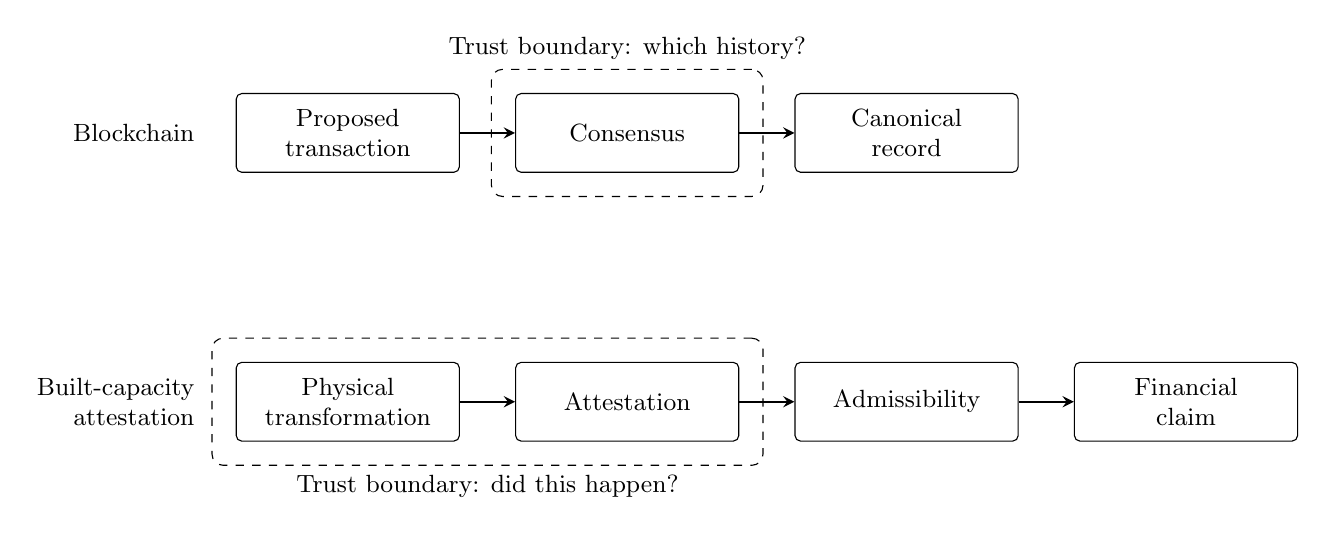
\begin{tikzpicture}[
    node distance=7mm and 7mm,
    box/.style={draw, rounded corners=2pt, align=center, minimum height=10mm, text width=26mm, font=\small},
    arr/.style={-stealth, thick}
]
\node[box] (tx) {Proposed\\transaction};
\node[box, right=of tx] (cons) {Consensus};
\node[box, right=of cons] (canon) {Canonical\\record};

\node[box, below=24mm of tx] (phys) {Physical\\transformation};
\node[box, right=of phys] (att) {Attestation};
\node[box, right=of att] (adm) {Admissibility};
\node[box, right=of adm] (claim) {Financial\\claim};

\draw[arr] (tx) -- (cons);
\draw[arr] (cons) -- (canon);
\draw[arr] (phys) -- (att);
\draw[arr] (att) -- (adm);
\draw[arr] (adm) -- (claim);

\node[draw, dashed, rounded corners, fit=(cons), inner sep=3mm,
      label=above:{\small Trust boundary: which history?}] {};
\node[draw, dashed, rounded corners, fit=(phys)(att), inner sep=3mm,
      label=below:{\small Trust boundary: did this happen?}] {};
\node[left=4mm of tx, font=\small, align=right] {Blockchain};
\node[left=4mm of phys, font=\small, align=right] {Built-capacity\\attestation};
\end{tikzpicture}
\caption{Two verification problems. In a blockchain the difficult question lies in the choice among proposed ledger histories. In built-capacity attestation it lies at the boundary between the physical event and the record, which consensus among replicas cannot cross.}
\label{fig:blockchain}
\end{figure}

This changes the location of the trust boundary. In a proof-of-work blockchain, substantial machinery is devoted to determining which proposed ledger history becomes authoritative. In a proof-of-stake system, authority over ordering is allocated through rules involving stake and protocol participation. In the present architecture, ordinary database replication may be sufficient for agreement over ledger state, and the difficult problem lies in the admissibility of the event that enters the ledger. For the same reason, the phrase proof of admissible improvement should not be understood as another consensus mechanism analogous to proof of work or proof of stake. It is an eligibility rule. A successful inspection does not select the canonical ledger history; it supplies evidence that a particular proposed transition is permitted. The two functions can be implemented independently. A jurisdiction could maintain the attestation system in an ordinary replicated database, publish cryptographic hashes or signed snapshots for audit \cite{merkle1987, laurie2013}, and denominate every resulting loan in an existing national currency, and nothing in the core design requires a token, a distributed consensus protocol, mining, staking, or a globally replicated state machine. The hierarchy of Section 11 makes the same point from the other direction, since its weakest levels require no new asset at all.

The two architectures also differ in their treatment of location. Public blockchains ordinarily seek to make the validity of a transaction independent of the physical location of the machine processing it, so that a transition is valid because it satisfies protocol rules wherever the validating node happens to stand. Built-capacity attestation has the opposite property, because location is constitutive of the claim. The tuple $(x,\tau,\kappa,\sigma,t)$ cannot discard $x$ without changing what is being asserted, and a compliant apartment built at one parcel cannot serve as evidence that an apartment was built at another. The ledger is consequently not merely distributed across space; it is about space.

A further difference concerns scarcity. Proof-of-work systems deliberately create an artificial computational scarcity to regulate participation in consensus, and proof-of-stake systems employ scarce protocol-native assets. The present system has no need to manufacture scarcity for this purpose. Its constraints arise from the physical and institutional process itself: land occupies locations, construction consumes materials and labour, transformations take time, inspections require observations, and structures depreciate. These constraints do not automatically produce a desirable money supply, as the preceding sections have shown, but they do mean that establishing that a physical transformation occurred does not call for an additional artificial scarcity.

Finally, the treatment of error is importantly different. An immutable record is not necessarily an accurate record. A mistaken or fraudulent inspection may need to be challenged without pretending that the original attestation never occurred, because loans or other actions may already have depended on it. The appropriate operation is therefore not silent deletion but a subsequent defeating entry,
\begin{equation}
a_0\longrightarrow a_1\longrightarrow\operatorname{retract}(a_1)\longrightarrow a_2,
\label{eq:retract}
\end{equation}
so that the historical ledger preserves both the original certification and its later defeat while the authoritative present state is computed from the history. Auditability requires append-only history \cite{helland2015}, but it does not require that every historical assertion remain authoritative forever. Retraction is thus an operation on the authority of an event and not on its existence, and this is the semantics the credit rule needs, a point developed in a companion essay on retraction as an operation.

The closest resemblance to blockchain is consequently the least important part of the design: both may employ cryptographic signatures, hashes, append-only records, and replicated storage. The substantive distinction lies in what those mechanisms are asked to establish. Blockchain consensus can answer the question of which ledger history the protocol accepted. A built-capacity attestation system must answer a different question: what happened at this place, under which rules, who warrants that it happened, and what claims may follow from it. That is a provenance and admissibility problem before it is a consensus problem. There is, moreover, a sense in which the design has less reason to use a blockchain precisely because it takes physical provenance seriously. Once the difficult information comes from inspectors, permits, parcels, construction records, and code editions, decentralized consensus does not eliminate the oracle of Section 5. It replicates what the oracle said.

\section{Depreciation, Destruction, and Built Capacity as Underwriting Information}

The reverse of issuance matters even more than issuance. A burned building, a condemned structure, a failed septic system, a withdrawn occupancy permit, or a flood reclassification reduces certified capacity, and the system cannot maintain the fiction that collateral persists because an old appraisal says so. This is a genuine advantage over appraisal-based collateral, but it creates a problem that conventional systems handle through balance-sheet losses borne by lenders and equity holders. In a system where money is issued against capacity, a reduction in capacity is a reduction in the backing of money already in circulation, and the question becomes who bears it.

Let capacity be treated as a stock with a flow description,
\begin{equation}
\frac{dC}{dt} \;=\; \iota(t) \;-\; \delta\,C(t) \;-\; \eta(t),
\label{eq:stock}
\end{equation}
where $\iota(t)$ is certified new improvement, $\delta$ is a depreciation rate reflecting ordinary physical aging, and $\eta(t)$ is discrete loss from fire, flood, condemnation, or regulatory withdrawal. If the monetary base is held at $\alpha\sum_x C(x)$ at all times, then a negative $dC/dt$ requires the destruction of money. But once money has escaped into general circulation, the destruction of a particular building does not identify which monetary units should disappear. Either some holders must be forced to surrender currency, which is a tax on holders of money for events they did not cause, or the currency must be redeemable against a diminishing base, which is a run waiting to happen, or the backing ratio $\alpha$ must be allowed to fall, which concedes that the money supply is not determined by capacity after all. The ordinary solution in credit systems is to attach the loss to a specific debtor through a loan contract, so that the destruction of the collateral is a loss to the borrower and lender who contracted for the exposure. This is the structure emphasized by credit theories of money, in which a unit of money is the counterpart of a specific debt \cite{mitchellinnes1913}. Issuance should therefore take the form of loans against certified improvement and not unattached creation of currency, with each loan amortizing at least as fast as its collateral depreciates.

This resolution changes the institutional identity of the design more than is usually acknowledged. What the ledger of certified capacity supplies is information about the existence, condition, and legal status of collateral, which is the substance of underwriting, and not a backing for the settlement medium. Built capacity works naturally as underwriting information and awkwardly as monetary backing. The treatment of maintenance follows the same logic. Under rule~\eqref{eq:stock}, a structure whose condition is maintained at the level of its original certification has $\delta C$ offset by $\iota$, and maintenance work is a form of improvement that counters decay. The accounting for this requires that the inspection regime certify not only discrete additions but the continued satisfaction of conditions, which is a recurring and costly activity. A system that supports credit generously for new construction and not for maintenance will create the incentive to build and abandon, and the stock of eligible collateral will expand over a housing stock whose average condition is declining.

\section{The Spatial Currency: Illustration, Difficulties, and Demotion}

The most unusual element of the first formulation is that the currency is spatially indexed. Units originating at nearby or infrastructurally connected locations exchange near par, and conversion across distant regions passes through a clearing mechanism, so that distance becomes part of monetary structure. This is distinct from both cryptocurrency, in which the ledger is deliberately placeless, and ordinary local currencies, in which a single geographic boundary separates a bounded circle of acceptance from the outside world \cite{blanc2011}. A family of conversion rules illustrates the idea. Let $d_G(u,v)$ be a shortest-path distance in the graph $G=(V,E)$ under an edge weighting that reflects infrastructural connection, and let a unit issued at $u$ exchange for units at $v$ at a rate
\begin{equation}
e_{uv} \;=\; \exp\!\bigl(-\lambda\, d_G(u,v)\bigr), \qquad \lambda\ge 0.
\label{eq:rate}
\end{equation}
The case $\lambda=0$ recovers a single fungible currency and $\lambda\to\infty$ recovers isolated local currencies. This family should be read as a symmetric penalty for distance. It forces $e_{uv}\le 1$ with $e_{uu}=1$, and with a symmetric $d_G$ it also gives $e_{uv}=e_{vu}$, so a unit is worth no more at another location than at its origin and the penalty is the same in both directions. If instead the intent were that units at different locations have different intrinsic strengths, the formula would need to be reworked with location-specific weights.

The family has one clean property, and it is worth stating because it is the only mathematical result the topology yields.

\begin{proposition}[No routing arbitrage]
If $d_G$ satisfies the triangle inequality, then for all vertices $u,v,w$ the conversion rule~\eqref{eq:rate} satisfies $e_{uw}\ge e_{uv}\,e_{vw}$, with equality if and only if $\lambda=0$ or $d_G(u,w)=d_G(u,v)+d_G(v,w)$.
\end{proposition}

\begin{proof}
By the triangle inequality $d_G(u,w)\le d_G(u,v)+d_G(v,w)$. Since $\lambda\ge 0$ and the exponential is increasing, $\exp(-\lambda d_G(u,w))\ge \exp(-\lambda[d_G(u,v)+d_G(v,w)]) = e_{uv}e_{vw}$. For $\lambda>0$ equality holds exactly when the triangle inequality is tight, that is, when $v$ lies on a shortest path from $u$ to $w$; for $\lambda=0$ both sides equal one.
\end{proof}

Direct conversion is therefore never worse than conversion through an intermediate vertex, so no agent profits by routing a conversion through a chain of regions, and equality occurs along shortest paths. This is a desirable property, but it is a statement about internal consistency of the rule and says nothing about whether the rule matches the rates at which goods and services in different regions actually exchange, and that is where the difficulty lies.

If conversion rates are fixed by a formula such as~\eqref{eq:rate}, any discrepancy between the formula and the market rate will be exploited. A concrete case makes the prediction explicit. Suppose one region undergoes a construction boom and issues heavily while a neighbouring region does not. Under a fixed conversion rule the units of the boom region are more abundant, while the formula equates them with the scarcer units of the neighbour. Agents will tender the abundant unit and hoard the scarce one, goods will flow toward the boom region where its units are accepted at par with something worth more, and the discrepancy will persist until the clearing mechanism is exhausted or the rate is adjusted. This is a Gresham dynamic in the literal sense. If conversion rates float, the system has recreated a set of regional currencies with a floating exchange rate, and the familiar results of optimum currency area theory \cite{mundell1961, mckinnon1963, kenen1969} apply. What those results imply here is that the appropriate value of $\lambda$ is not a property of the physical graph but depends on labour mobility between the regions, on the capacity of fiscal transfers to absorb asymmetric shocks, and on the symmetry of the shocks the regions face. These are empirical questions about specific regional economies, and they cannot be settled by the geometry of roads and utilities.

The historical cases that are usually invoked in favour of spatially bounded media support less than is sometimes claimed. The Swiss WIR network is a firm-to-firm credit clearing system, and the evidence that its demand rose when conventional credit contracted \cite{stodder2009} bears on the countercyclical behaviour of mutual credit among firms. It is not evidence about a currency backed by built capacity. The Wörgl experiment of the early 1930s was a local stamp scrip scheme built on Gesell's proposal for demurrage-bearing money \cite{gesell1916}, a design that Fisher promoted as a response to hoarding and deflation \cite{fisher1933}, and its monetary logic, in which holding the medium is penalized, is quite different from capacity backing. Each is relevant by analogy to the question of how a locally bounded medium circulates and how it relates to a monetary authority, and neither supplies support for any particular backing rule.

These difficulties suggest that the spatial currency should be demoted from the core of the design to an optional extension. The ledger already preserves location without making the settlement asset location-dependent: the arrangement is located collateral together with a fungible settlement medium. The graph $G$ can then do different work. Let $w_{uv}$ measure settlement or infrastructural dependence between $u$ and $v$, and let the graph govern collateral eligibility, regional exposure limits, clearing fees, systemic concentration, infrastructure dependence, and reserve requirements. A lender then holds perfectly ordinary claims denominated in an ordinary currency while the ledger records where each claim originates. Defining the exposure of a portfolio to a node $v$ as the share of its claims whose collateral depends on $v$,
\begin{equation}
h_v \;=\; \frac{\sum_{k} c_k\,\mathbf{1}[k \text{ depends on } v]}{\sum_{k} c_k},
\label{eq:exposure}
\end{equation}
where $c_k$ is the size of claim $k$, a prudential rule can bound $h_v$ for every vertex: no more than a stated fraction of a portfolio may depend on one municipal water system, one floodplain, or one regional construction market. The topology becomes useful for systemic-risk analysis without requiring a unit issued in one town to trade against a unit issued in another. The result is a stronger use of the location idea than the first formulation: location becomes a property of the provenance of a claim and not a property of the unit of account.

\section{The Reformulation: Transformation as the Primitive}
\label{sec:repair}

The preceding sections suggest where the first formulation went wrong. It treated certified capacity as the primitive object against which money is issued, and nearly every difficulty found traces to that choice. The stock has no numeraire, it decays, its legal definition is a legislative variable, and its attribution between site and structure is conventional. The repair replaces the stock by an event.

\begin{principle}[Transformation primitive]
Certified built capacity is better treated as ledger state derived from attested transformations than as the primitive object against which money is issued.
\end{principle}

\noindent The ledger consists of the append-only sequence of indexed attestations of Definition~1, each carrying a location, a transformation, a code edition, a signed inspection record, and a time. Certified capacity at a location is a derived quantity, computed from that sequence under a stated edition, and it can be recomputed under any other edition for which the transformation records suffice. The monetary quantity is likewise derived from the attested event: the system does not say that a building contains a given number of monetary units, but that a particular, inspectable transformation occurred here, under these rules, at this time, and qualifies for this amount of credit.

\begin{figure}[htbp]
\centering
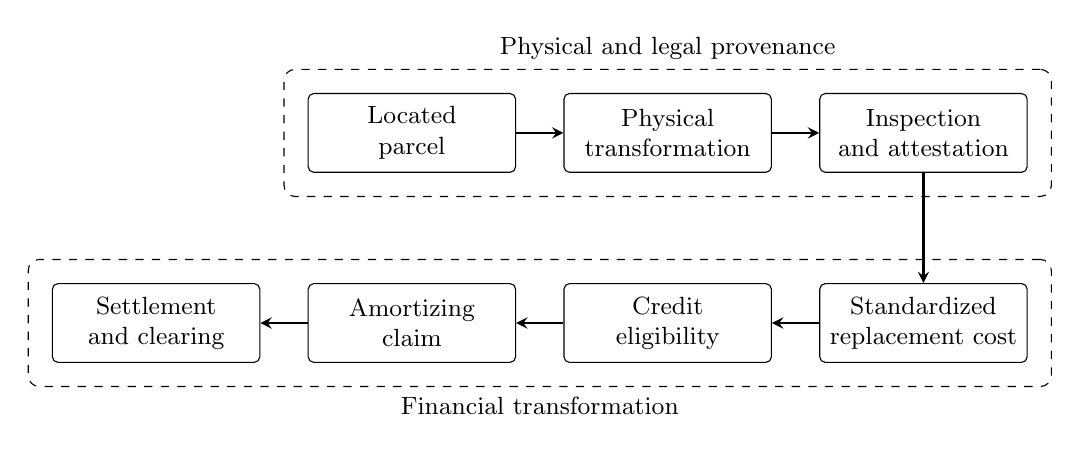
\begin{tikzpicture}[
    node distance=6mm and 6mm,
    box/.style={draw, rounded corners=2pt, align=center, minimum height=10mm, text width=24mm, font=\small},
    arr/.style={-stealth, thick}
]
\node[box] (parcel) {Located\\parcel};
\node[box, right=of parcel] (transform) {Physical\\transformation};
\node[box, right=of transform] (inspect) {Inspection\\and attestation};
\node[box, below=14mm of inspect] (value) {Standardized\\replacement cost};
\node[box, left=of value] (credit) {Credit\\eligibility};
\node[box, left=of credit] (loan) {Amortizing\\claim};
\node[box, left=of loan] (clearing) {Settlement\\and clearing};
\draw[arr] (parcel) -- (transform);
\draw[arr] (transform) -- (inspect);
\draw[arr] (inspect) -- (value);
\draw[arr] (value) -- (credit);
\draw[arr] (credit) -- (loan);
\draw[arr] (loan) -- (clearing);
\node[draw, dashed, rounded corners, fit=(parcel)(transform)(inspect), inner sep=3mm,
      label=above:{\small Physical and legal provenance}] {};
\node[draw, dashed, rounded corners, fit=(value)(credit)(loan)(clearing), inner sep=3mm,
      label=below:{\small Financial transformation}] {};
\end{tikzpicture}
\caption{The repaired architecture. Location enters through the provenance of the underlying transformation and not through the denomination of the settlement medium.}
\label{fig:architecture}
\end{figure}


The credit that a transformation qualifies for requires a measure of its reproduction cost, and that measure is doing a great deal of work. It is at once the valuation mechanism, the bridge to the numeraire, and the basis for issuance. Writing it as a function of $\tau$ alone would conceal that construction costs vary geographically, over time, and with the code edition. Labour costs, transportation costs, materials availability, climate-specific requirements, remoteness, and economies of scale all affect what it costs to reproduce a given transformation, and a square metre of compliant construction in a remote northern community cannot meaningfully have the same reproduction cost as one in a large southern city. The cost function is therefore written
\begin{equation}
\rho(\tau,\,x,\,t,\,\kappa),
\label{eq:rho}
\end{equation}
with $x$ capturing geographically varying real input costs, $t$ the price date, and $\kappa$ the applicable code edition. The permitted credit for an attested transformation is
\begin{equation}
\Delta M(\tau) \;=\; \alpha\,\rho(\tau,x,t,\kappa)\,\mathbf{1}\bigl[\tau \text{ realized and certified}\bigr],
\label{eq:issue}
\end{equation}
with no credit for zoning changes, none for site-value changes, and credit for maintenance transformations at the same rate as for new construction. Two meanings of location are separated by this formulation, and the separation should be defended carefully because the first formulation left them entangled. Location as a production condition, meaning the fact that producing the same physical transformation costs different amounts in different places, legitimately enters $\rho$. Location as scarcity rent, meaning the additional sum a purchaser will pay merely to possess one coordinate and not another, is the quantity $S_x$ and does not enter issuance. A house in a remote northern community can support a different standardized valuation from an otherwise identical house in a large southern city because moving materials, employing labour, and meeting climate requirements genuinely cost different amounts, and nothing about this reintroduces speculative land value.

\begin{figure}[htbp]
\centering
\hyphenpenalty=10000 \exhyphenpenalty=10000
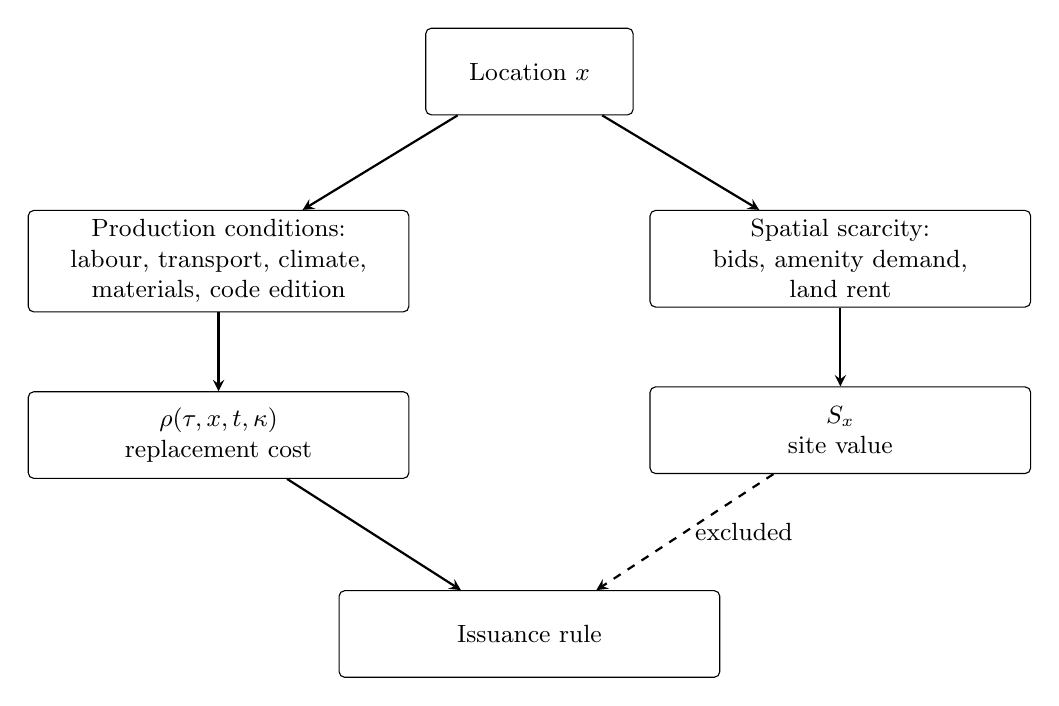
\begin{tikzpicture}[
    node distance=10mm and 12mm,
    box/.style={draw, rounded corners=2pt, align=center, minimum height=11mm, text width=46mm, font=\small},
    arr/.style={-stealth, thick}
]
\node[box, text width=24mm] (location) {Location $x$};
\node[box, below left=12mm and 2mm of location] (production) {Production conditions:\\ labour, transport, climate,\\ materials, code edition};
\node[box, below right=12mm and 2mm of location] (rent) {Spatial scarcity:\\ bids, amenity demand,\\ land rent};
\node[box, below=of production] (rho) {$\rho(\tau,x,t,\kappa)$\\ replacement cost};
\node[box, below=of rent] (site) {$S_x$\\ site value};
\node[box, below=20mm of $(rho)!0.5!(site)$] (issue) {Issuance rule};
\draw[arr] (location) -- (production);
\draw[arr] (location) -- (rent);
\draw[arr] (production) -- (rho);
\draw[arr] (rent) -- (site);
\draw[arr] (rho) -- (issue);
\draw[arr, dashed] (site) -- node[midway, right, font=\small] {excluded} (issue);
\end{tikzpicture}
\caption{Two meanings of location. Geographic variation in the real cost of reproducing a transformation may enter the replacement-cost index, while scarcity rent and transaction-price appreciation are excluded from the issuance rule.}
\label{fig:two-location-effects}
\end{figure}


Three results follow.

\begin{proposition}[Insensitivity to site bids]
Under rule~\eqref{eq:issue}, with $\rho$ determined from construction input costs independently of transaction prices for the parcel, the credit originated against a parcel is invariant under any change in $S_x$ that is not accompanied by a realized, certified transformation of the parcel.
\end{proposition}

\begin{proof}
By~\eqref{eq:issue}, $\Delta M(\tau)$ is nonzero only when $\tau$ is realized and certified, and its value depends on $\tau$, on the location's input costs, on the price date, and on the code edition. A change in $S_x$ without a transformation yields no $\tau$, hence $\Delta M=0$. Because $\rho$ is determined independently of the parcel's transaction price, no other channel carries $S_x$ into $\Delta M$.
\end{proof}

\begin{proposition}[Legislative expansion does not issue]
Let $A_{\mathrm{permitted}}(x)$ be the legally permitted floor area at $x$ and $A_{\mathrm{realized}}(x)$ the floor area of certified transformations at $x$. Under rule~\eqref{eq:issue},
\[
\Delta A_{\mathrm{permitted}}>0,\quad \Delta A_{\mathrm{realized}}=0 \quad\Longrightarrow\quad \Delta M=0 .
\]
\end{proposition}

\begin{proof}
A change in permitted area alters the set of transformations that may later be certified but is not itself a transformation. With $\Delta A_{\mathrm{realized}}=0$ there is no new realized and certified $\tau$, so the indicator in~\eqref{eq:issue} vanishes.
\end{proof}

\begin{figure}[htbp]
\centering
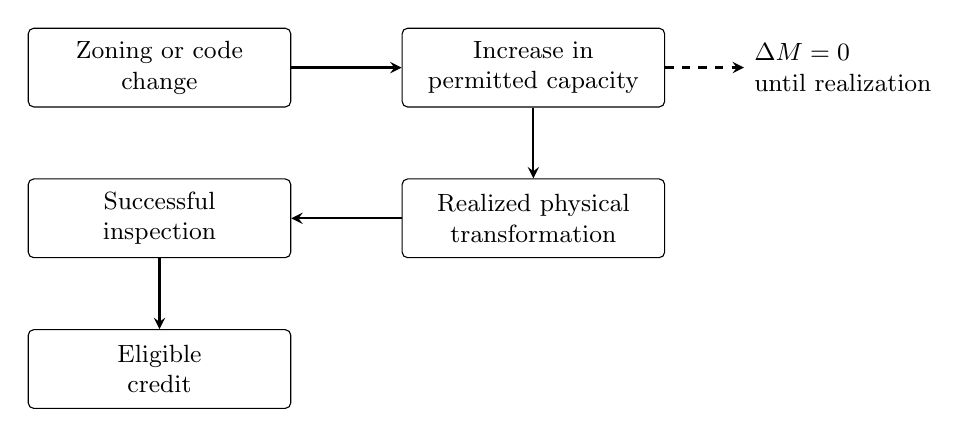
\begin{tikzpicture}[
    node distance=9mm and 14mm,
    box/.style={draw, rounded corners=2pt, align=center, minimum height=10mm, text width=31mm, font=\small},
    arr/.style={-stealth, thick},
    noissue/.style={-stealth, dashed, thick}
]
\node[box] (law) {Zoning or code\\change};
\node[box, right=of law] (permitted) {Increase in\\permitted capacity};
\node[box, below=of permitted] (construction) {Realized physical\\transformation};
\node[box, left=of construction] (inspection) {Successful\\inspection};
\node[box, below=of inspection] (credit) {Eligible\\credit};
\draw[arr] (law) -- (permitted);
\draw[arr] (permitted) -- (construction);
\draw[arr] (construction) -- (inspection);
\draw[arr] (inspection) -- (credit);
\draw[noissue] (permitted.east) -- ++(10mm,0) node[right, align=left, font=\small] {$\Delta M=0$\\until realization};
\end{tikzpicture}
\caption{Permitted capacity and realized capacity. A legislative change enlarges the feasible state space but does not itself constitute an issuance event.}
\label{fig:permitted-realized}
\end{figure}


The first proposition is nearly tautological, and the observation that matters is what it leaves open. The tautology is informative only if $\rho$ can be constructed independently enough of local conditions that scarcity rent does not leak into it, which is a question about how the index is built: whether national, regional, or input-price weighted, how it is updated, and who audits it. The second proposition establishes the narrower result that the legislative expansion of the state space cannot by itself produce credit, which closes the avenue by which a municipality could print backing by redrawing a map.

The third result concerns a feedback that the repair does not remove. Replacement-cost issuance creates its own endogenous loop. If credit stimulates construction, construction raises the demand for labour and materials, those prices rise, the published reproduction-cost index rises, and identical subsequent transformations qualify for greater credit:
\begin{equation}
\text{credit}\uparrow \;\to\; \text{construction demand}\uparrow \;\to\; \rho\uparrow \;\to\; \Delta M_{\mathrm{eligible}}\uparrow .
\label{eq:rhofeed}
\end{equation}
This replacement-cost feedback is importantly different from the collateral-price feedback the system removes. The land-price loop runs through the bids of purchasers for a fixed supply of coordinates, and nothing physical need restrain it. The replacement-cost loop runs through the prices of actual scarce productive inputs, and its gain is limited by the supply of labour and materials and by the elasticity of the construction sector, which varies widely across places \cite{saiz2010}. It is nonetheless endogenous, and the design must treat the index as a variable that the system itself moves, for example by smoothing it over a long window, by indexing to input costs excluding the system's own marginal demand where that can be measured, or by tying $\alpha$ to the index's rate of change. That the loop is real and bounded, and not absent, is the correct description.

\section{Governance: Rule-Based Issuance Is Not Discretion-Free Issuance}

Once attestation and valuation are identified as the critical institutions, governance becomes endogenous to the theory and cannot be set aside as administration. Someone chooses the code edition $\kappa$, constructs the index $\rho$, accredits inspectors, hears challenges, decides when an attestation is defeated, and determines the consequences of fraud. Someone also sets the backing fraction $\alpha$, and, if a clearing graph is retained, the parameters that govern it and the bounds on exposure in~\eqref{eq:exposure}. Each of these is a decision with monetary consequences, and calling them technical does not remove the authority they exercise; it only places a monetary authority inside several technical offices. The general principle is that
\begin{equation}
\text{rule-based issuance} \;\neq\; \text{discretion-free issuance}.
\label{eq:discretion}
\end{equation}
Discretion has not been eliminated by tying credit to verified transformations. It has migrated upstream into the definition, measurement, and certification of eligible transformations. This observation matters because it blocks a rhetorical move to which the design is prone, the claim that credit backed by objective physical facts is thereby free of the judgment that characterizes ordinary central banking. The facts are objective only relative to a definition, a measurement procedure, and an accreditation process, and each of those is a site where interest, error, and capture can enter.

The political-economy questions are accordingly part of the specification, not a supplement to it. Who appoints and rotates inspectors, and who pays for audit? Who publishes the index $\rho$, and what prevents the entities that benefit from higher credit eligibility from influencing it? By what procedure is the code edition amended, and how are legacy structures treated? Who may challenge an attestation, on what evidence, and with what standing? Who bears the cost when an attestation is defeated after credit has been extended? A design that cannot answer these questions has not specified a monetary or credit institution, however clean its formalism. The honest statement is that the design relocates the locus of discretion and makes it more legible, since the points at which judgment is exercised are enumerated in the ledger's structure, but legibility is not elimination.

\begin{figure}[htbp]
\centering
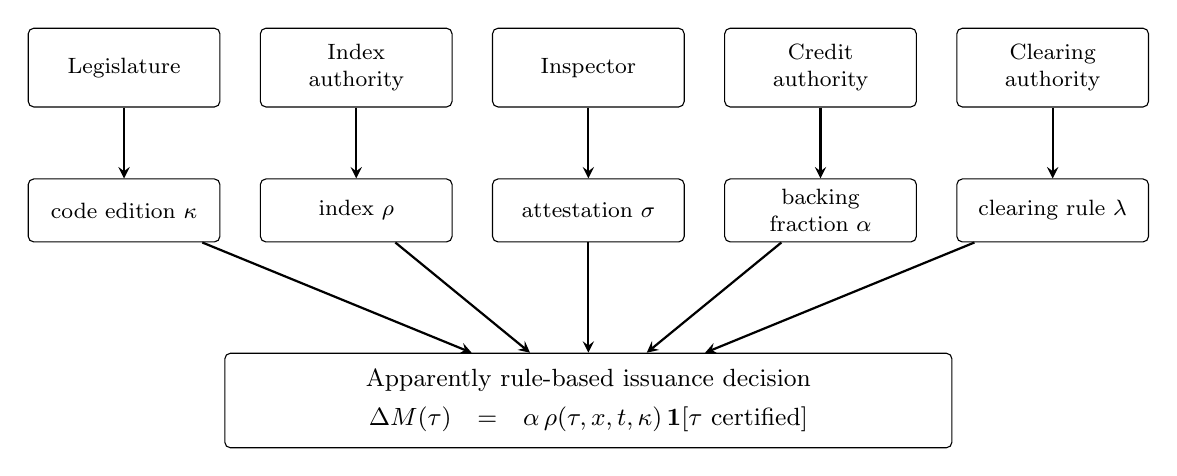
\begin{tikzpicture}[
    node distance=5mm and 5mm,
    auth/.style={draw, rounded corners=2pt, align=center, minimum height=10mm, text width=22mm, font=\footnotesize},
    par/.style={draw, rounded corners=2pt, align=center, minimum height=8mm, text width=22mm, font=\footnotesize},
    arr/.style={-stealth, thick}
]
\node[auth] (leg) {Legislature};
\node[auth, right=of leg] (idx) {Index\\authority};
\node[auth, right=of idx] (ins) {Inspector};
\node[auth, right=of ins] (cre) {Credit\\authority};
\node[auth, right=of cre] (clr) {Clearing\\authority};
\node[par, below=9mm of leg] (kappa) {code edition $\kappa$};
\node[par, below=9mm of idx] (rho) {index $\rho$};
\node[par, below=9mm of ins] (sigma) {attestation $\sigma$};
\node[par, below=9mm of cre] (alpha) {backing fraction $\alpha$};
\node[par, below=9mm of clr] (lambda) {clearing rule $\lambda$};
\foreach \a/\b in {leg/kappa, idx/rho, ins/sigma, cre/alpha, clr/lambda}
    \draw[arr] (\a) -- (\b);
\node[draw, rounded corners=2pt, align=center, minimum height=12mm, text width=90mm, font=\small,
      below=14mm of sigma] (issue) {Apparently rule-based issuance decision\\[1mm] $\Delta M(\tau)=\alpha\,\rho(\tau,x,t,\kappa)\,\mathbf 1[\tau\text{ certified}]$};
\foreach \b in {kappa, rho, sigma, alpha, lambda}
    \draw[arr] (\b) -- (issue);
\end{tikzpicture}
\caption{Where discretion resides. Five distinct authorities fix the parameters and inputs of an apparently rule-based issuance decision, so that rule-based issuance is not discretion-free issuance.}
\label{fig:discretion}
\end{figure}


\section{A Nested Hierarchy and Its Institutional Neighbours}

The reformulation reveals that the design is not a single system but a family. Define a sequence of institutional commitments, each extending the previous one:
\begin{equation}
\begin{aligned}
\mathcal L_0 &: \text{attestation registry},\\
\mathcal L_1 &: \mathcal L_0+\text{standardized collateral eligibility},\\
\mathcal L_2 &: \mathcal L_1+\text{transformation-linked credit issuance},\\
\mathcal L_3 &: \mathcal L_2+\text{graph-structured clearing},\\
\mathcal L_4 &: \mathcal L_3+\text{spatially differentiated units}.
\end{aligned}
\label{eq:hierarchy}
\end{equation}
The important analytical property is nesting. One need not establish the viability of $\mathcal L_4$ to justify $\mathcal L_1$, and the failure of a stronger level does not undermine a weaker one. The weakest level, $\mathcal L_0$, is simply a located ledger of attested transformations. The level $\mathcal L_1$ uses that ledger to define which loans qualify as secured by admissible collateral and with what haircut. The level $\mathcal L_2$ introduces credit creation tied to the ledger's events, and $\mathcal L_3$ adds the exposure-bounding and clearing structure of Section 8. The level $\mathcal L_4$ is the spatially differentiated currency of the first formulation, and the analysis above gives reasons to expect it to be the weakest link. The most defensible limiting case is $\mathcal L_1$ in its simplest form, and it requires no new money whatsoever: a jurisdiction could maintain the attestation registry, compute standardized replacement-cost increments, and permit ordinary lending denominated in an existing currency against those increments, with the same insensitivity to site bids and without the demand-for-money problem of Section 3.

\begin{figure}[htbp]
\centering
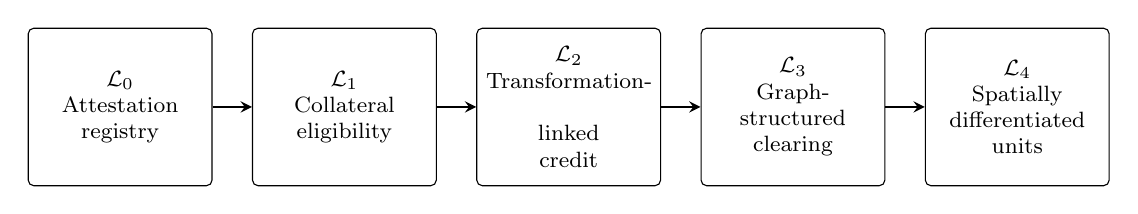
\begin{tikzpicture}[
    node distance=5mm,
    level/.style={draw, rounded corners=2pt, align=center, minimum height=20mm, text width=21mm, font=\footnotesize},
    arr/.style={-stealth, thick}
]
\node[level] (l0) {$\mathcal L_0$\\Attestation\\registry};
\node[level, right=of l0] (l1) {$\mathcal L_1$\\Collateral\\eligibility};
\node[level, right=of l1] (l2) {$\mathcal L_2$\\Transformation-\\linked\\credit};
\node[level, right=of l2] (l3) {$\mathcal L_3$\\Graph-structured\\clearing};
\node[level, right=of l3] (l4) {$\mathcal L_4$\\Spatially\\differentiated units};
\draw[arr] (l0) -- (l1);
\draw[arr] (l1) -- (l2);
\draw[arr] (l2) -- (l3);
\draw[arr] (l3) -- (l4);
\end{tikzpicture}
\caption{Nested institutional commitments. Each level adds a stronger claim to the preceding architecture. The viability of a lower level does not depend on the viability of the stronger levels to its right.}
\label{fig:institutional-levels}
\end{figure}


Two institutional comparisons make the position of this design more exact. The first is with the cadastre, discussed above: the registry is a cadastre extended by transformation records, and what is new is the coupling of that registry to a credit rule. The second is with the collateral frameworks already used by central banks and regulated lenders, which maintain eligibility schedules, valuation haircuts, collateral classes, and risk adjustments \cite{bindseil2004, gorton2012}. The distinctive step here is to replace some market-value-dependent recognition of collateral with recognition that depends on the provenance of a certified transformation. This is a narrower and more exactly located innovation than the creation of a new money. The design is not a full-reserve or narrow-banking scheme in the sense of Fisher's \emph{100\% Money} \cite{fisher1935} and its modern restatements \cite{benes2012}, since it does not separate deposit creation from lending; the comparison to that tradition is useful chiefly for locating the separation between the creation of the settlement medium and the allocation of credit, which the reformulation also maintains by leaving the settlement medium fungible.

The distributional questions are best stated in the vocabulary that loans supply, and that vocabulary should replace the looser use of seigniorage found in discussions of money creation. Seigniorage proper is the difference between the face value of money and its cost of production, accruing to the issuer \cite{buiter2007}, and the redistribution that arises because newly created purchasing power reaches particular recipients first is closer to what is called the Cantillon effect \cite{cantillon1755}. In a loan-based system there are four distinct questions: who receives the initial credit, who receives the interest income, who absorbs default losses, and whether the public captures any rent from granting the privilege of issuance. Credit issued at the point of construction favours those who build, and a rule that declines to extend credit against site appreciation disadvantages those whose wealth is held in appreciated land. The second consequence is intended and is the Georgist core of the design. The first deserves scrutiny, since the scale of the transfer to builders depends on $\alpha$, and a public share in the proceeds, through fees or a retained interest, is a design variable and not an afterthought.

\section{Illustrative Simulations}
\label{sec:sims}

The arguments above concern the structure of feedback and incidence under alternative rules, and four small simulations are included to display those structures. They are dimensionless computational experiments and are not calibrated to any housing, construction, or lending data. Their parameter values were chosen to make the mechanisms visible, not estimated, and their outputs follow from the assumptions built into them. What each figure shows is therefore the presence or absence of a channel under a stated rule, and not the empirical magnitude of that channel in any jurisdiction. All four figures are regenerated by a single script, \texttt{simulate.py}, which uses only NumPy and Matplotlib. The parameters are collected in Table~\ref{tab:params}, and periods are an abstract unit of time.

\begin{table}[htbp]
\centering
\small
\begin{tabular}{@{}c p{3.3cm} p{8.6cm}@{}}
\hline
Figure & Rule & Parameters \\
\hline
1 & Collateral-price regime & price growth $g=0.012$, credit effect on price $\beta=0.10$, collateral sensitivity $\gamma=0.75$ \\
1 & Transformation regime & improvement flow $0.008+0.002\sin(k/4)$ per period \\
2 & Capacity stock & depreciation $\delta=0.012$, new build $0.018$, destruction $0.28$ at period 24, $\alpha=0.65$ \\
2 & Amortizing loans & amortization $0.035$, origination $0.030$, impairment $0.16$ at period 24 \\
3 & Replacement cost & base build $0.020$, boom amplitude $0.030$ centred at period 20 (width 7), $\alpha=0.70$, cost sensitivity $0.75$, reversion $0.18$ \\
4 & Clearing graph & path A--B--C, clearing rate $0.16$, claims per period: A $0.11$ in periods 10 to 24 and $0.025$ otherwise, B $0.020$, C $0.015$ \\
\hline
\end{tabular}
\caption{Parameters of the dimensionless illustrative simulations.}
\label{tab:params}
\end{table}

\paragraph{Price feedback versus transformation-linked issuance.}
Figure~\ref{fig:feedback} compares two stylized regimes. In the collateral-price regime the price $P_k$ and the credit stock $M_k$ evolve as $P_{k+1}=P_k+g+\beta\max(M_k-1,0)$ and $M_{k+1}=1+\gamma(P_{k+1}-1)$, so that credit is a linear function of price appreciation and excess credit raises prices in turn. Substituting the second relation into the first, the deviation $P_k-1$ obeys a recursion whose growth rate is $\beta\gamma$, the product of the price response to credit and the sensitivity of credit to collateral value. The loop therefore produces geometric acceleration for any positive product, and the curve bends upward for exactly the reason that the property-price feedback of Section~2 does. In the transformation regime credit increases only by the realized improvement flow, which does not depend on $P$, and the series is close to linear. The comparison is a statement about loop gain and not about the level of either series: the second regime was built to have no channel from price to credit, so its insensitivity is an assumption, and the content of the figure is the difference in structure that the assumption produces.

\begin{figure}[htbp]
\centering
\includegraphics[width=0.88\linewidth]{figures/fig1_collateral_vs_transformation.png}
\caption{Dimensionless illustrative simulation of collateral-price-linked credit and transformation-linked credit. The simulation exhibits the presence or absence of a direct price-to-credit feedback channel and does not estimate its empirical magnitude.}
\label{fig:feedback}
\end{figure}

\paragraph{A destruction shock.}
Figure~\ref{fig:destruction} applies a capacity-destruction event to two designs. Certified capacity evolves as $C_{k+1}=C_k+\iota-\delta C_k-\eta_k$, with a single discrete loss $\eta$, and under the literal stock-backed rule the base is $\alpha C_k$ and must contract with it. Under the loan design the impairment is attached to the claims exposed to the destroyed capacity, and the settlement medium itself is unaffected. The two series are different objects, since one is an economy-wide base and the other is the outstanding stock of transformation-linked claims, and their heights should not be compared as if they measured the same quantity. The magnitude of the loan loss in particular is set by the assumed impairment parameter, and the figure is not evidence that loans lose less in general. The relevant contrast is incidence. Under the stock rule the contraction is borne by every holder of the medium irrespective of any exposure to the destroyed buildings, whereas under the loan rule it falls on the parties to the impaired contracts, which is the argument of Section~7 in numerical form.

\begin{figure}[htbp]
\centering
\includegraphics[width=0.88\linewidth]{figures/fig2_destruction_shock.png}
\caption{Dimensionless illustrative simulation of a capacity-destruction shock. The first series is a literal stock-backed monetary base and the second is outstanding transformation-linked claims, which are not the whole money supply. The comparison concerns who bears the loss and not the relative size of the loss.}
\label{fig:destruction}
\end{figure}

\paragraph{Replacement-cost feedback.}
Figure~\ref{fig:rho} isolates the residual feedback of Section~9. Issuance satisfies $\Delta M_k=\alpha\,\rho_k\,\iota_k$, with $\iota_k$ the realized building flow, and in the endogenous case the index relaxes toward a target that rises with excess building, $\rho_{k+1}=\rho_k+r(\rho^{*}_k-\rho_k)$, where $\rho^{*}_k=1+s\,(\iota_k-\iota_0)^{+}/\iota_0$. During the boom the endogenous series pulls ahead of the fixed-index benchmark, and because the credit stock is cumulative the gap persists after the index has reverted, so credit extended at inflated reproduction cost is not retired by the cost's later decline. Two limits of the experiment should be stated. The boom is imposed from outside, so the figure illustrates the transmission from construction pressure to eligible credit and not the full loop in~\eqref{eq:rhofeed}, which would also require an elasticity of construction to credit that is not modeled. And the index reverts toward its base by assumption, so the bounded character of the effect, in contrast to the geometric growth in the first figure, is again a property of the specification. It is nevertheless the specification suggested by the argument that this loop runs through scarce inputs.

\begin{figure}[htbp]
\centering
\includegraphics[width=0.88\linewidth]{figures/fig3_replacement_cost_feedback.png}
\caption{Dimensionless illustrative simulation of residual replacement-cost feedback during an exogenous building boom. The simulation illustrates the existence and persistence of the channel and does not estimate its size.}
\label{fig:rho}
\end{figure}

\paragraph{Clearing on a graph.}
Figure~\ref{fig:clearing} uses three regions on the path A--B--C. Region A originates more claims during a temporary boom, and clearing flows between adjacent regions are proportional to differences in their outstanding regional claim balances. The balances are provenance accounts for claims, and the settlement medium is assumed fungible, in keeping with the demotion of the spatial currency in Section~8. The boom region's balance rises fastest and then relaxes toward those of its neighbours as clearing proceeds, while the adjacent region is raised before the distant one, so the spatial ordering of the shock is visible in the order of arrival. The experiment demonstrates a graph used for recording and relaxing exposure, which is the use proposed in Section~8. It does not model prices, goods flows, or conversion rates, and so says nothing about the arbitrage and Gresham dynamics of a spatially differentiated currency, which remain arguments and are not simulated here.

\begin{figure}[htbp]
\centering
\includegraphics[width=0.88\linewidth]{figures/fig4_spatial_clearing.png}
\caption{Dimensionless illustrative simulation of regional claim balances on a three-node clearing graph. Money is treated as fungible and only the provenance of claims is spatially indexed. The simulation is not an empirical model.}
\label{fig:clearing}
\end{figure}

Taken together, the four experiments support the qualitative claims made in the text and nothing beyond them. They show that removing a price channel changes the feedback structure, that incidence differs between stock backing and loan structures, that a cost-index channel remains and is persistent in level, and that a graph can carry exposure without carrying a unit of account. Any statement about size or timing in a particular economy would require the data and calibration that these experiments deliberately do not use.

\section{What Remains Unshown}

The reformulation establishes that the idea can be stated coherently, not that it is desirable. The demand-for-money problem is avoided at the weaker levels by leaving the settlement medium to its existing issuer and is mitigated by the loan structure at $\mathcal L_2$, but nothing here guarantees that the volume of eligible transformations matches the volume of settlement needed in an economy. The treatment of capital other than buildings, such as machinery, software, and skill, is absent, so the credit rule favours one class of capital in an economy where most of the productive stock is of other kinds. The legal-tender and taxation questions, which determine whether any new medium is accepted, are untouched, and the historical record of complementary currencies suggests that acceptance by the taxing authority is often more decisive than the design of the backing. And the empirical question of how large the effects of the proposed channels would be is not addressed by any derivation in this essay; any quantitative claim would require data on construction costs, permit flows, and lending in specific jurisdictions that are not supplied here.

\section{Conclusion}

The idea that a ledger entry must ultimately point back to somewhere is a sound design constraint, and the design has the merit of taking it seriously. Formalization shows that the idea begins as an exotic theory of money and ends as a theory of credit admissibility, and this is not merely a retreat. Following the movement from property-backed money, through capacity-backed money, to transformation-backed credit, and finally to an attestation-based collateral architecture, one can say exactly which components survive decomposition and where they belong institutionally. The distinction between creating capacity and bidding up its price identifies a real defect in the collateral channel of property finance and survives as the insensitivity of credit eligibility to site bids. The use of building codes as an ontology of verifiable physical facts survives with the qualification that codes are legislated, revisable, and subject to the incentives that accompany any rewarded measure. The spatial topology survives as a property of the provenance and exposure of claims and not as a property of the unit of account.

The result can be stated in two sentences. Location belongs naturally in the provenance of a financial claim, but it does not follow that location should belong in the denomination of money. Likewise, building codes can determine whether a transformation is admissible collateral without determining the quantity of money an economy should possess. What replaces the first question of how much money a building should contain is the question of what monetary claims a verified transformation should be permitted to originate, and the answer depends less on the physics of buildings than on the institutions that define, measure, and certify the transformations. A public ledger of attested physical transformations, indexed to code editions, supporting standardized replacement-cost-based credit against realized improvement, is worth specifying in full, and the weakest version of it can be built with no new currency at all.

\begin{thebibliography}{99}
\bibitem{arnott1979} R.~J. Arnott and J.~E. Stiglitz, ``Aggregate Land Rents, Expenditure on Public Goods, and Optimal City Size,'' \emph{Quarterly Journal of Economics} 93(4), 1979.
\bibitem{becker1968} G.~S. Becker, ``Crime and Punishment: An Economic Approach,'' \emph{Journal of Political Economy} 76(2), 1968.
\bibitem{benes2012} J.~Bene\v{s} and M.~Kumhof, ``The Chicago Plan Revisited,'' IMF Working Paper WP/12/202, 2012.
\bibitem{bernanke1989} B.~S. Bernanke and M.~Gertler, ``Agency Costs, Net Worth, and Business Fluctuations,'' \emph{American Economic Review} 79(1), 1989.
\bibitem{bindseil2004} U.~Bindseil, \emph{Monetary Policy Implementation: Theory, Past, and Present}, Oxford University Press, 2004.
\bibitem{blanc2011} J.~Blanc, ``Classifying `CCs': Community, Complementary and Local Currencies' Types and Generations,'' \emph{International Journal of Community Currency Research} 15(A), 2011.
\bibitem{buiter2007} W.~H. Buiter, ``Seigniorage,'' \emph{Economics: The Open-Access, Open-Assessment E-Journal} 1, 2007.
\bibitem{buneman2001} P.~Buneman, S.~Khanna, and W.-C. Tan, ``Why and Where: A Characterization of Data Provenance,'' in \emph{Database Theory (ICDT 2001)}, Springer, 2001.
\bibitem{campbell1979} D.~T. Campbell, ``Assessing the Impact of Planned Social Change,'' \emph{Evaluation and Program Planning} 2(1), 1979.
\bibitem{cantillon1755} R.~Cantillon, \emph{Essai sur la nature du commerce en g\'en\'eral}, 1755.
\bibitem{castro1999} M.~Castro and B.~Liskov, ``Practical Byzantine Fault Tolerance,'' in \emph{Proceedings of the Third Symposium on Operating Systems Design and Implementation (OSDI)}, 1999.
\bibitem{desoto2000} H.~de~Soto, \emph{The Mystery of Capital}, Basic Books, 2000.
\bibitem{fisher1933} I.~Fisher, \emph{Stamp Scrip}, Adelphi, 1933.
\bibitem{fisher1935} I.~Fisher, \emph{100\% Money}, 1935.
\bibitem{george1879} H.~George, \emph{Progress and Poverty}, 1879.
\bibitem{gesell1916} S.~Gesell, \emph{Die nat\"urliche Wirtschaftsordnung}, 1916 (English edition: \emph{The Natural Economic Order}).
\bibitem{glaeser2003} E.~L. Glaeser and J.~Gyourko, ``The Impact of Building Restrictions on Housing Affordability,'' \emph{Federal Reserve Bank of New York Economic Policy Review} 9(2), 2003.
\bibitem{goodhart1975} C.~A.~E. Goodhart, ``Problems of Monetary Management: The U.K. Experience,'' in \emph{Papers in Monetary Economics}, Reserve Bank of Australia, 1975.
\bibitem{gorton2012} G.~Gorton and A.~Metrick, ``Securitized Banking and the Run on Repo,'' \emph{Journal of Financial Economics} 104(3), 2012.
\bibitem{gyourko2008} J.~Gyourko, A.~Saiz, and A.~Summers, ``A New Measure of the Local Regulatory Environment for Housing Markets: The Wharton Residential Land Use Regulatory Index,'' \emph{Urban Studies} 45(3), 2008.
\bibitem{helland2015} P.~Helland, ``Immutability Changes Everything,'' \emph{ACM Queue} 13(9), 2015.
\bibitem{jorda2016} \`O.~Jord\`a, M.~Schularick, and A.~M. Taylor, ``The Great Mortgaging: Housing Finance, Crises and Business Cycles,'' \emph{Economic Policy} 31(85), 2016.
\bibitem{kenen1969} P.~B. Kenen, ``The Theory of Optimum Currency Areas: An Eclectic View,'' in R.~A. Mundell and A.~K. Swoboda (eds.), \emph{Monetary Problems of the International Economy}, University of Chicago Press, 1969.
\bibitem{kiyotaki1997} N.~Kiyotaki and J.~Moore, ``Credit Cycles,'' \emph{Journal of Political Economy} 105(2), 1997.
\bibitem{knoll2017} K.~Knoll, M.~Schularick, and T.~Steger, ``No Price Like Home: Global House Prices, 1870--2012,'' \emph{American Economic Review} 107(2), 2017.
\bibitem{lamport1982} L.~Lamport, R.~Shostak, and M.~Pease, ``The Byzantine Generals Problem,'' \emph{ACM Transactions on Programming Languages and Systems} 4(3), 1982.
\bibitem{laurie2013} B.~Laurie, A.~Langley, and E.~Kasper, ``Certificate Transparency,'' RFC 6962, 2013.
\bibitem{law1705} J.~Law, \emph{Money and Trade Considered, with a Proposal for Supplying the Nation with Money}, 1705.
\bibitem{mckinnon1963} R.~I. McKinnon, ``Optimum Currency Areas,'' \emph{American Economic Review} 53(4), 1963.
\bibitem{merkle1987} R.~C. Merkle, ``A Digital Signature Based on a Conventional Encryption Function,'' in \emph{Advances in Cryptology (CRYPTO '87)}, 1987.
\bibitem{mian2011} A.~Mian and A.~Sufi, ``House Prices, Home Equity-Based Borrowing, and the US Household Leverage Crisis,'' \emph{American Economic Review} 101(5), 2011.
\bibitem{mints1945} L.~W. Mints, \emph{A History of Banking Theory}, University of Chicago Press, 1945.
\bibitem{mitchellinnes1913} A.~Mitchell-Innes, ``What Is Money?'' \emph{Banking Law Journal}, 1913.
\bibitem{muller2018} J.~Z. Muller, \emph{The Tyranny of Metrics}, Princeton University Press, 2018.
\bibitem{mundell1961} R.~A. Mundell, ``A Theory of Optimum Currency Areas,'' \emph{American Economic Review} 51(4), 1961.
\bibitem{nakamoto2008} S.~Nakamoto, ``Bitcoin: A Peer-to-Peer Electronic Cash System,'' 2008.
\bibitem{oates1997} W.~E. Oates and R.~M. Schwab, ``The Impact of Urban Land Taxation: The Pittsburgh Experience,'' \emph{National Tax Journal} 50(1), 1997.
\bibitem{saiz2010} A.~Saiz, ``The Geographic Determinants of Housing Supply,'' \emph{Quarterly Journal of Economics} 125(3), 2010.
\bibitem{sargent1982} T.~J. Sargent and N.~Wallace, ``The Real-Bills Doctrine versus the Quantity Theory: A Reconsideration,'' \emph{Journal of Political Economy} 90(6), 1982.
\bibitem{schularick2012} M.~Schularick and A.~M. Taylor, ``Credit Booms Gone Bust: Monetary Policy, Leverage Cycles, and Financial Crises, 1870--2008,'' \emph{American Economic Review} 102(2), 2012.
\bibitem{scott1998} J.~C. Scott, \emph{Seeing Like a State}, Yale University Press, 1998.
\bibitem{stigler1971} G.~J. Stigler, ``The Theory of Economic Regulation,'' \emph{Bell Journal of Economics and Management Science} 2(1), 1971.
\bibitem{stodder2009} J.~Stodder, ``Complementary Credit Networks and Macroeconomic Stability: Switzerland's Wirtschaftsring,'' \emph{Journal of Economic Behavior \& Organization} 72(1), 2009.
\bibitem{strathern1997} M.~Strathern, ```Improving Ratings': Audit in the British University System,'' \emph{European Review} 5(3), 1997.
\bibitem{tirole1986} J.~Tirole, ``Hierarchies and Bureaucracies: On the Role of Collusion in Organizations,'' \emph{Journal of Law, Economics, and Organization} 2(2), 1986.
\end{thebibliography}

\end{document}
